%%%%%%%%%%%%%%%%%%%%%%%%%%%%%%%%%%%%%%%%%
% Beamer Presentation
% LaTeX Template
% Version 1.0 (10/11/12)
%
% This template has been downloaded from:
% http://www.LaTeXTemplates.com
%
% License:
% CC BY-NC-SA 3.0 (http://creativecommons.org/licenses/by-nc-sa/3.0/)
%
%%%%%%%%%%%%%%%%%%%%%%%%%%%%%%%%%%%%%%%%%

%----------------------------------------------------------------------------------------
%	PACKAGES AND THEMES
%----------------------------------------------------------------------------------------

\documentclass{beamer}

\mode<presentation> {

% The Beamer class comes with a number of default slide themes
% which change the colors and layouts of slides. Below this is a list
% of all the themes, uncomment each in turn to see what they look like.

%\usetheme{default}
%\usetheme{AnnArbor}
%\usetheme{Antibes}
%\usetheme{Bergen}
%\usetheme{Berkeley}
\usetheme{Berlin}
%\usetheme{Boadilla}
%\usetheme{CambridgeUS}
%\usetheme{Copenhagen}
%\usetheme{Darmstadt}
%\usetheme{Dresden}
%\usetheme{Frankfurt}
%\usetheme{Goettingen}
%\usetheme{Hannover}
%\usetheme{Ilmenau}
%\usetheme{JuanLesPins}
%\usetheme{Luebeck}
%\usetheme{Madrid}
%\usetheme{Malmoe}
%\usetheme{Marburg}
%\usetheme{Montpellier}
%\usetheme{PaloAlto}
%\usetheme{Pittsburgh}
%\usetheme{Rochester}
%\usetheme{Singapore}
%\usetheme{Szeged}
%\usetheme{Warsaw}

% As well as themes, the Beamer class has a number of color themes
% for any slide theme. Uncomment each of these in turn to see how it
% changes the colors of your current slide theme.

%\usecolortheme{albatross}
%\usecolortheme{beaver}
%\usecolortheme{beetle}
%\usecolortheme{crane}
%\usecolortheme{dolphin}
%\usecolortheme{dove}
%\usecolortheme{fly}
%\usecolortheme{lily}
%\usecolortheme{orchid}
%\usecolortheme{rose}
%\usecolortheme{seagull}
\usecolortheme{seahorse}
%\usecolortheme{whale}
%\usecolortheme{wolverine}

\setbeamertemplate{footline} % To remove the footer line in all slides uncomment this line
%\setbeamertemplate{footline}[page number] % To replace the footer line in all slides with a simple slide count uncomment this line

\setbeamertemplate{navigation symbols}{} % To remove the navigation symbols from the bottom of all slides uncomment this line
}

\usepackage{graphicx} % Allows including images
\usepackage{booktabs} % Allows the use of \toprule, \midrule and \bottomrule in tables


\usepackage{amsmath}
\usepackage{amsthm}
\usepackage{amssymb}
\usepackage{amsfonts}
\usepackage{mathrsfs}
\usepackage{bbm}
\usepackage{color}
\usepackage{hyperref}
\usepackage{url}
\usepackage{graphicx}
\usepackage{xcolor}
\usepackage{tikz}
\usepackage{tikz-cd}
\usepackage{enumerate}
\usepackage{wrapfig}

\usepackage{color}
\usepackage{xcolor}
\usepackage{hyperref}
\hypersetup{
	colorlinks,
	linkcolor={red!50!black},
	citecolor={blue!50!black},
	urlcolor={blue!80!black}
}
\usepackage{hyperref}
\usepackage{url}

\usepackage[english]{babel}
\usepackage[autostyle, english = american]{csquotes}
%\MakeOuterQuote{"}
\usepackage{datetime}

\graphicspath{{img/}}
\newcommand{\E}{\ensuremath{\mathbb{E}}}
\newcommand{\cvar}{\ensuremath{\operatorname{CVaR}}}

%----------------------------------------------------------------------------------------
%	TITLE PAGE
%----------------------------------------------------------------------------------------

\title[Short title]{Generalizing expectation to general risk measures} % The short title appears at the bottom of every slide, the full title is only on the title page

\author{Yuxi Liu} % Your name
\institute[ANU] % Your institution as it will appear on the bottom of every slide, may be shorthand to save space
{
Australian National University \\ % Your institution for the title page
\medskip
%\textit{} % Your email address
}

\newdate{date}{28}{10}{2019}
\date{\displaydate{date}}
%\date{\today} % Date, can be changed to a custom date

\begin{document}

\begin{frame}
\titlepage
\end{frame}

\begin{frame}
\frametitle{Overview}
\tableofcontents
\end{frame}

%----------------------------------------------------------------------------------------
%	PRESENTATION SLIDES
%----------------------------------------------------------------------------------------

%------------------------------------------------
\section{General level (13 min)}
%------------------------------------------------

\begin{frame}
\frametitle{An investment problem (4 min)}
	If you have some cash, and you'd like to purchase some stocks, hold for a year, then sell them. How do you maximize gain? That is, minimize loss?
	\pause
	
	Let there be $N$ stocks to pick from, and your strategy is to invest a portion $x_i$ of the cash into stock i. Then your strategies are defined by a vector $x = (x_1, ... x_N)$\pause
	
	Let the loss from the investment be $L = L(x)$. Since investment outcome is uncertain, $L(x)$ is a random variable. We would like to find some $x$ that "minimizes" $L(x)$.\pause
	
	$L(x)$ is random, so it can't be minimized directly. The usual solution is to minimize its expectation:

	$$x^* = \arg\min_x\E(L(x))$$
\end{frame}

\begin{frame}
	\frametitle{Expectation can be dangerous (7 min)}
	\only<1>{
	Minimizing expectation could be, however, dangerous when there is a small chance of catastrophe.
	
	~
	
	Consider an example from finance.
	}
	\only<2>{
	Collapse of Long-Term Capital Management cost \$4 billion.
	
	\begin{figure}
		\centering
		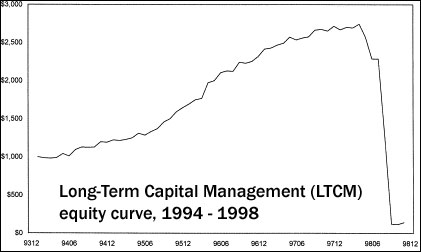
\includegraphics[width=0.8\textwidth]{ltcm}
	\end{figure}
	}
%	\only<3>{
%		The expectation of temperature rise is $3 ^\circ$C, but the small chance of warming $6 ^\circ$C is very dangerous.
%	\begin{figure}
%		\centering
%		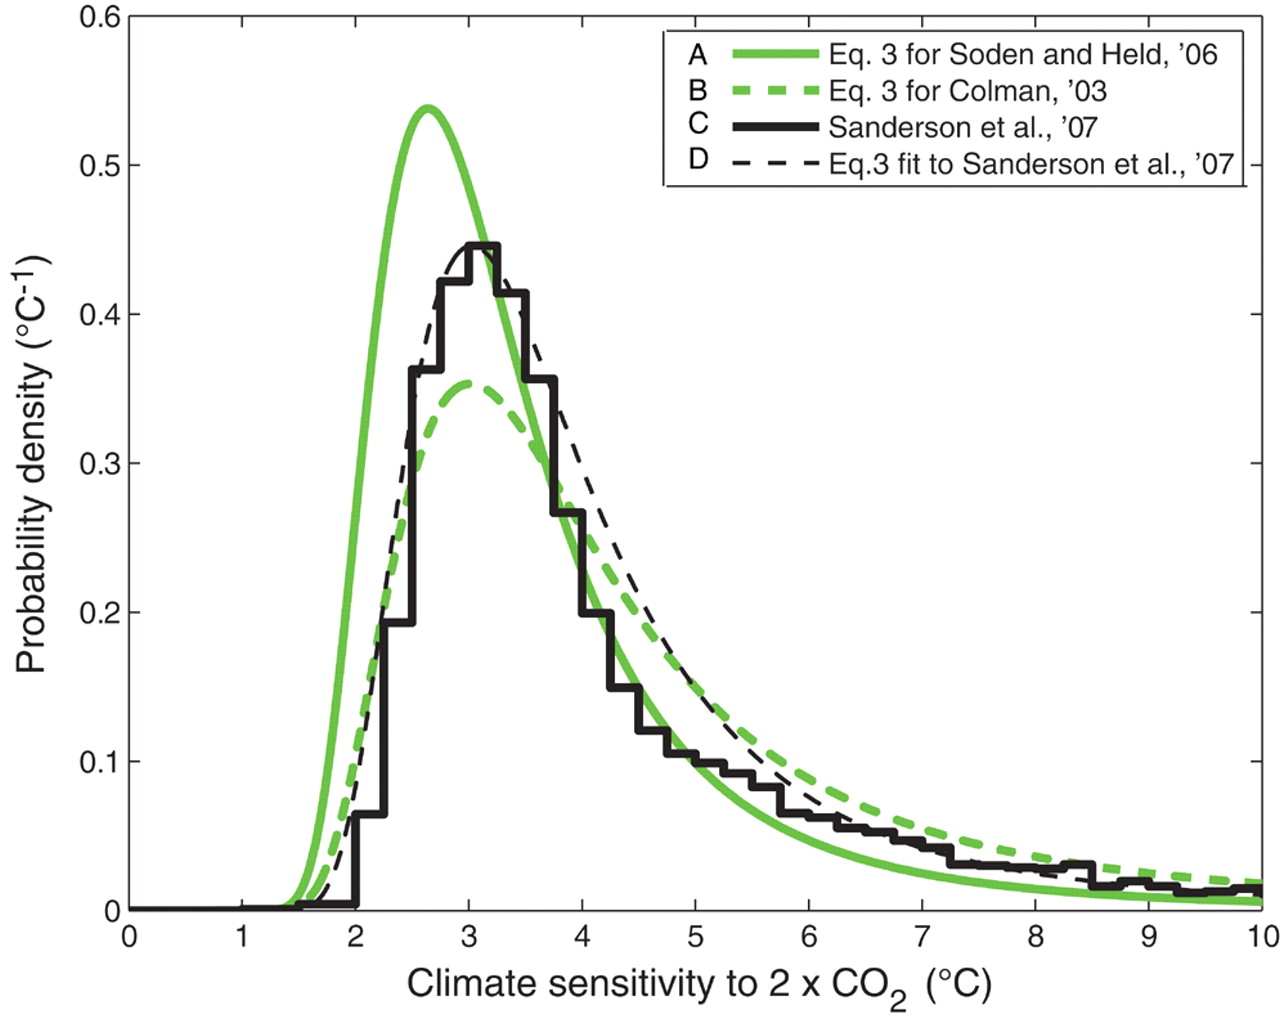
\includegraphics[width=0.6\textwidth]{climate_tail}
%	\end{figure}
%
%	{\scriptsize Figure from “Why Is Climate Sensitivity so Unpredictable?" (Roe and Baker, 2007)}
%	}
\end{frame}

\begin{frame}
	\frametitle{Controlling the tail (13 min)}
	To deal with the dangerous long tail, we can control its tail directly.\pause
	
	~
	
	Consider a normally distributed random variable $X\sim \mathcal{N}(\mu, \sigma^2)$. 
	
	$\mathcal{N}$ denotes a normal distribution with mean $\mu$ and variance $\sigma^2$.\pause
	
	~
	
	Then, instead of the expectation, we consider the tail expectation:
	$$ \E(X | X > q_\alpha(X))
	$$
	where $q_\alpha(X)$ is the $\alpha$-quantile of $X$.
\end{frame}

%------------------------------------------------



%------------------------------------------------
\section{Undergrad probability level (10 min)}
%------------------------------------------------

\begin{frame}
	\frametitle{CVaR: Conditional value at risk (18 min)}
	
	\begin{block}{Definition of CVaR}
		For any random variable $X$, and $0\le\alpha<1$, 
		$$
		\cvar_\alpha(X) = \E(X|X > q_\alpha(X))
		$$
		The $\alpha = 1$ case is special:
		$\cvar_1(X) = \sup(X)$
	\end{block}\pause

	\begin{example}
		Let $X$ be uniform over $[0, 1]$, then,
		$$q_\alpha(X) = \alpha, \cvar_\alpha(X) = \frac 12 (1+\alpha)$$
	\end{example}
\end{frame}

\begin{frame}
\frametitle{Discrete approximation (23 min)}
	Given random variable $X$, we can construct an approximation of $X$ by sampling the first $n$ terms of its IID process $X_1, X_2, ... X_n$. Then let $L_n$ be a random variable that is equal to $X_i$ with probability $1/n$. \pause
	
	~
	
	If $n$ is big, and $X$ is "nice", then $L_n$ should be "similar" to $X$. For example, we should have 
	$$\E(L_n) = \frac 1 n \sum_{i=1}^n X_i \approx \E(X)$$
	
	{\scriptsize Side remark: This is essentially "bootstrapping" from statistics.}
	
\end{frame}

\section{Graduate probability level (15 min)}

\begin{frame}
	\frametitle{Central limit theorem (33 min)}
	\only<1>{
	Intuitively, the central limit theorem states that for any $X$ with variance $\sigma^2$, we have
	
	$$\mathbb{E}(L_n) = \frac 1 n \sum_{i=1}^n X_i \approx \mathbb{E}(X) + \frac{1}{\sqrt n} \mathcal{N}(0, \sigma^2) + o\left(n^{-1/2} \right)$$
	
	That is, $\sqrt{n}(\E(L_n) -\E(X))$ converges to $\mathcal{N}(0, \sigma^2)$ in distribution.
	
	This suggests the generalization
	
	\begin{block}{Central limit theorem for CVaR}
		For any $X$ with finite variance, there exists some function $\sigma: [0, 1) \to [0, \infty)$, such that
		$$\cvar_\alpha(L_n) \approx \cvar_\alpha(X) + \frac{1}{\sqrt n} \mathcal{N}(0, \sigma(\alpha)^2) + o\left(n^{-1/2} \right)$$
	\end{block}
	}	\only<2>{
	\begin{block}{Central limit theorem for CVaR}
	Since $L_n$ is a mixture of $X_1, ... X_n$, we have 
	$$\cvar_\alpha(L_n) \approx \frac{1}{(1-\alpha)n}\sum_{i = 1}^{(1-\alpha)n} X_{(i)} $$
	where $X_{(i)}$ is the i-th greatest among all $X_1, ... X_n$.\pause
	
	~
	
	We proved that $\sigma(\alpha)^2$ equals
	$$
	\mathbb{V}\left(\frac 1{1-\alpha} (X - q_\alpha(X))^+\right)
	$$
	\end{block}
}
\end{frame}

\begin{frame}
	\frametitle{Numerical experiments (38 min)}
	
	For $X$ uniform over $\{0, 1, 2\}$, we generated trials of $\cvar_\alpha(L_{1000})$, 
	\only<1>{and graphed theoretical vs actual $\sigma(\alpha)^2$:
	
	\begin{figure}
		\centering
		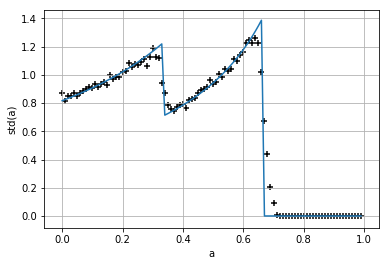
\includegraphics[width=0.7\textwidth]{discrete_0_1_2_std}
	\end{figure}
	What happens at the "jumps", like $\alpha = 1/3$?}
	\only<2>{
		\begin{figure}
			\centering
			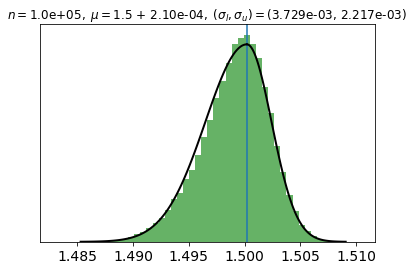
\includegraphics[width=0.75\textwidth]{cvar_boundary_behavior_discrete_0_1_2}
		\end{figure}
	The distribution of $\cvar_{1/3}(L_n)$ becomes "mixed Gaussian"!
	}
	

\end{frame}

\section{Grader level (10 min)}

\begin{frame}
	\frametitle{Proof of central limit theorem (43 min)}
	The proof of the theorem proceeded in 4 steps:
	\begin{enumerate}
		\item Use the G\"artner–Ellis theorem to calculate the result as an integral equation. \pause
		\item Solve the equation when $X$ is a mixture of uniform distributions over intervals on the real line. \pause
		\item Take the limit so that $X$ has discrete distribution. \pause
		\item A general $X$ distribution is takes as the limit of a sequence of discrete distributions.
	\end{enumerate}
\end{frame}

\begin{frame}
	\frametitle{Strong law of large numbers (48 min)}
	Finally, we have the remarkable generalization
	\begin{block}{Uniform strong law of large numbers for general risk measures}
	Let $X$ be a random variable with bounded range.
	
	\alert{With probability 1}, for any $m$ probability distribution over $[0, 1]$, the risk measure defined by 
	$$\mathcal{F}(X) = \int_0^1 \cvar_\alpha(X) dm(\alpha)$$
	gives
	$$\lim_n\mathcal{F}(L_n) = \mathcal{F}(X)$$
	\end{block}
	Prove the base case with G\"artner-Ellis, then "bootstrap" from it. 
\end{frame}


%------------------------------------------------

\begin{frame}{Conclusion (50 min)}
\begin{enumerate}
	\item Expectation is not necessarily the best for describing the relevant behaviors of a random variable. \pause
	\item Minimizing the CVaR of risk, instead of the expectation, allows more prudent planning. \pause
	\item There are remarkable generalizations to basic theorems of probability theory, once expectation is replaced with CVaR.
\end{enumerate}
\end{frame}

%------------------------------------------------

%\begin{frame}
%\Huge{\centerline{The End}}
%\end{frame}

%----------------------------------------------------------------------------------------


\end{document}